\subsection{平方根中间分布的有限步 Hellinger 进展}

平方根 target 把冻结学生与教师的平方根概率加权后归一化，而不是直接对概率作算术平均。记 $u=\sqrt q$、$v=\sqrt T$、$a=u^\top v$、$w=1-\eta$，则
\begin{equation}
 \sqrt{m_{1/2,\eta}}=\frac{wu+\eta v}{\sqrt Z},\qquad
 Z=w^2+\eta^2+2w\eta a.
 \label{eq:power-half-normalized-chord}
\end{equation}
$u,v$ 在正单位球面上。归一化的正线性组合位于两者张成的二维平面及短圆弧上，因而是 Fisher--Rao 路径的一个参数化；$\eta$ 通常不是弧长比例。对 $q=T$，该路径恒定。

\begin{theorem}[平方根 target 的精确亲和度与收缩]
\label{thm:power-half-discrete-contraction}
采用不带 $1/2$ 因子的 $H^2(q,T)=\sum_a(\sqrt{q_a}-\sqrt{T_a})^2=2(1-a)$。精确平方根更新满足
\begin{align}
 a^+&=\sum_a\sqrt{m_aT_a}=\frac{wa+\eta}{\sqrt Z},\\
 H^2(m,T)&\le(1-\eta)H^2(q,T).
 \label{eq:power-half-discrete-progress}
\end{align}
因此固定教师下反复精确更新得到 $H^2(q_N,T)\le(1-\eta)^NH^2(q_0,T)$。目标与锚点的平方根夹角 $\vartheta_{qm}$ 还满足
\begin{equation}
 \cos\vartheta_{qm}=\frac{w+\eta a}{\sqrt Z},\qquad
 \sin^2\vartheta_{qm}=\frac{\eta^2(1-a^2)}Z.
\end{equation}
这些都是精确分布更新的性质，不要求对 teacher 概率指定统一下界。
\end{theorem}

\begin{proof}
式~\eqref{eq:power-half-normalized-chord} 与 $v$ 内积直接给出 $a^+$。由于 $a\le1$，$Z\le(w+\eta)^2=1$，且 $wa+\eta>0$，有 $a^+\ge wa+\eta$。所以 $1-a^+\le w(1-a)$，乘以二即得 Hellinger 收缩。每轮重复应用即可得 $N$ 步界。与 $u$ 内积得到第二个夹角的余弦；再计算 $Z-(w+\eta a)^2=\eta^2(1-a^2)$，得到正弦平方。
\end{proof}

几何端点在同一 Hellinger 指标下没有严格小于一的分布无关单步收缩因子。固定 $0<\eta<1$，取 $q_\epsilon=(\epsilon,1-\epsilon)$、$T=(1/2,1/2)$，则几何 target 的第一坐标为
\begin{equation}
 m_{0,\eta,1}
 =\frac{\epsilon^{1-\eta}}{\epsilon^{1-\eta}+(1-\epsilon)^{1-\eta}}
 \longrightarrow0.
\end{equation}
因此 $q_\epsilon$ 与其几何 target 都趋于 $(0,1)$，两者到 $T$ 的 $H^2$ 都趋于 $2(1-1/\sqrt2)>0$，收缩比趋于一。平方根点的 $(1-\eta)$ 因子加强了相对于几何端点的统一全局 Hellinger 保证；教师附近的局部因子仍与其他形状相同，见后一定理。

\begin{corollary}[平方根精确外层的几何噪声界]
\label{cor:power-half-geometric-noise}
固定教师和 $0<\eta<1$，反复执行精确平方根 target。令 $V_n=\Var_{q_n}A_{1/2,\eta}(T/q_n)$，则
\begin{align}
 V_n&\le\frac{4H^2(q_n,T)}{(1-\eta)^2}
 \le\frac{4(1-\eta)^nH^2(q_0,T)}{(1-\eta)^2},\\
 \sum_{n=0}^\infty V_n&\le\frac{4H^2(q_0,T)}{\eta(1-\eta)^2}
 \le\frac8{\eta(1-\eta)^2}.
\end{align}
若 score 范数统一不超过 $S$，中心化教师梯度的协方差 trace 满足相应右侧乘以 $S^2$ 的界。
\end{corollary}

\begin{proof}
第~\ref{thm:center-advantage-variance}~定理给出 $V_n\le D_{1/2}(T\Vert q_n)/[(1/2)(1-\eta)^2]$。用 $D_{1/2}=2H^2$ 与前一定理的 Hellinger 收缩得到第一式。对 $n\ge0$ 求和，几何级数为 $1/\eta$；最后使用 $H^2\le2$。梯度二阶矩由 score 范数界控制。
\end{proof}

这比一般 MD 的 $O(1/N)$ 监督方差界更明确：平方根精确外层具有同一有界误差量驱动的几何噪声上界，累计上界不依赖可能任意大的初始 KL。它仍要求固定前缀和精确 target 更新；实际 BPO 误差会另外进入进展界。

\begin{figure}[H]
 \centering
 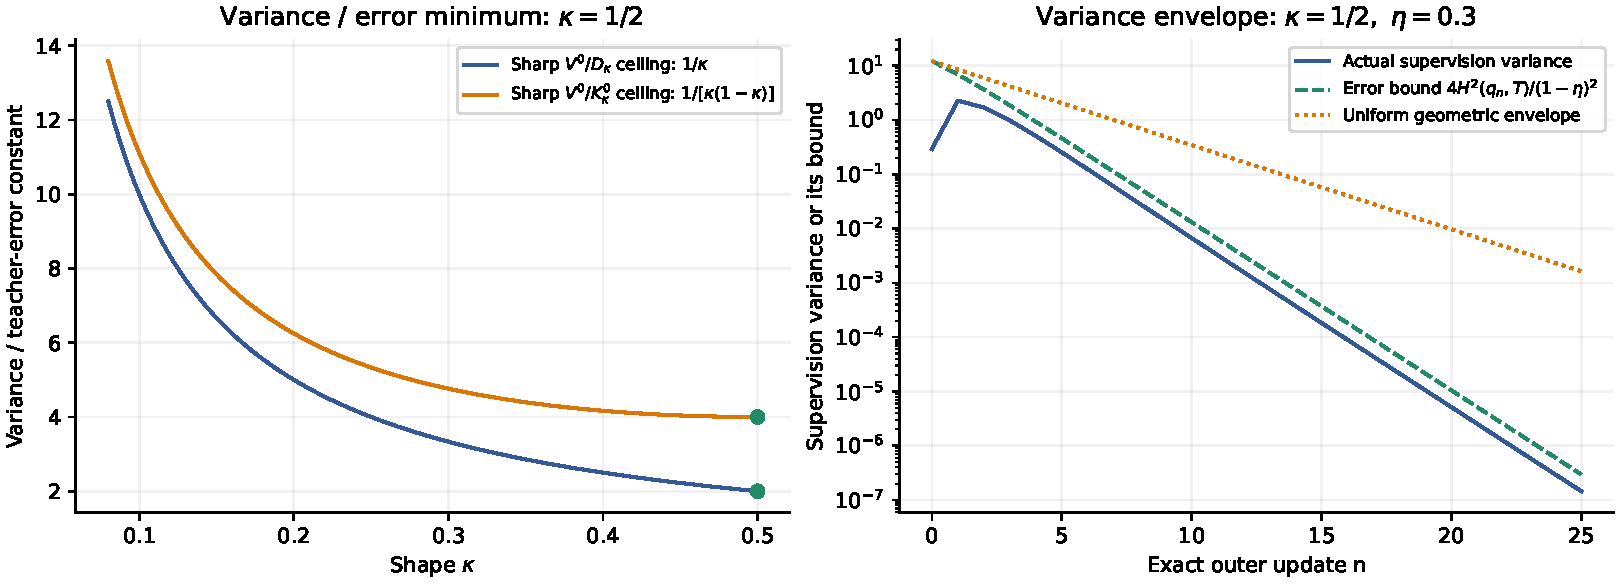
\includegraphics[width=\textwidth]{../../results/chapter9-restructure/relative-noise-and-convergence.pdf}
 \caption{左图以相对教师误差的锐噪声常数选择形状，两个准则均在 $\kappa=1/2$ 最小。右图对 $q_0=(0.999,0.001)$、$T=(0.05,0.95)$、$\eta=0.3$ 做精确平方根迭代。Hellinger 驱动的方差上界和统一几何包络下降，实际标量方差在第一步却增大。几何包络控制收敛过程，并不保证实际方差逐步单调。}
 \label{fig:power-relative-noise-convergence}
\end{figure}

\subsection{所有形状共享局部收敛率}

\begin{theorem}[幂均值的局部展开与共同收缩因子]
\label{thm:power-common-local-rate}
固定正支持教师 $T$、$0<\eta<1$、$0\le\kappa\le1$。令 $q=T+\epsilon h$，其中 $\sum h_a=0$、$h\ne0$，并使全部 $\epsilon h_a/T_a$ 一致趋零。记 $w=1-\eta$、$S_h=\sum_ah_a^2/T_a$，则
\begin{equation}
 m_a=T_a+w\epsilon h_a
 +\frac{(\kappa-1)w\eta}{2}\epsilon^2
       \left(\frac{h_a^2}{T_a}-T_aS_h\right)+O(\epsilon^3).
 \label{eq:power-second-order-target}
\end{equation}
若凸生成函数 $g$ 在一附近三阶可微且 $g''(1)>0$，则
\begin{equation}
 \frac{D_g(m\Vert T)}{D_g(q\Vert T)}
 =(1-\eta)^2+O(\epsilon).
 \label{eq:power-local-divergence-rate}
\end{equation}
因此在同一局部评价散度下，平方根形状没有优于其他形状的一阶概率误差收缩率。固定 $q,\eta$ 的 BPO logits Hessian 同样不因 $\kappa$ 改善。
\end{theorem}

\begin{proof}
对 $\kappa>0$，先展开
\begin{equation}
 (1-\eta)q_a^\kappa+\eta T_a^\kappa
 =T_a^\kappa\left[1+w\kappa\epsilon\frac{h_a}{T_a}
 +\frac{w\kappa(\kappa-1)}2\epsilon^2\frac{h_a^2}{T_a^2}
 +O(\epsilon^3)\right].
\end{equation}
再使用 $(1+x)^{1/\kappa}$ 的二阶展开，未归一化幂均值为
\begin{equation}
 \widetilde m_a=T_a+w\epsilon h_a
 +\frac{(\kappa-1)w\eta}{2}\epsilon^2\frac{h_a^2}{T_a}+O(\epsilon^3).
\end{equation}
求和时一次项消失，得到 $Z=1+[(\kappa-1)w\eta/2]\epsilon^2S_h+O(\epsilon^3)$。除以 $Z$ 即得第一式。几何端点可以直接展开 $q_a^wT_a^\eta$，得到同一式子中 $\kappa=0$ 的结果。

将 $g$ 加上线性项使 $g'(1)=0$ 不改变散度。Taylor 展开给出 $D_g(q\Vert T)=g''(1)\epsilon^2S_h/2+O(\epsilon^3)$。用 $m-T=w\epsilon h+O(\epsilon^2)$ 再展开，得到 $D_g(m\Vert T)=g''(1)w^2\epsilon^2S_h/2+O(\epsilon^3)$。$g''(1)S_h>0$，相除得到第二式。BPO 的曲率结论由第~\ref{sec:power-bpo-algorithm}~节的精确二次型给出。
\end{proof}

\subsection{形状选择取决于明确的评价标准}

\begin{center}
\small
\begin{tabular}{p{55mm}p{35mm}p{54mm}}
\toprule
评价标准 & 结论 & 条件与含义\\
\midrule
小步监督的分布无关有限方差 & $0<\kappa\le1/2$ & $1/2$ 是该区间的最大形状\\
小步方差相对教师误差的最坏比值 & $\kappa=1/2$ & $V\le2D_{1/2}=4H^2$，常数最优\\
最坏小步标量方差／Fisher 速度 & $\kappa_\star\simeq0.441928$ & 锐值 $3.527275$；平方根为 4\\
相同 Fisher 速度下的 reverse KL 局部下降 & $\kappa=0$ & 最陡确定性方向；无统一尾部界\\
相同 Fisher 速度下的 forward KL 局部下降 & $\kappa=1$ & 最陡确定性方向；小步最坏方差发散\\
当前学生采样的幂散度拟合噪声常数 & $\kappa_{\mathrm{fit}}=1/2$ & 拟合形状的最优性，不是 BPO target 最优性\\
固定 $q,\eta$ 的 BPO 条件数 & 对所有 $\kappa$ 相同 & 形状只改变 target 与初始残差\\
数学任务正确率与 NN 优化效率 & 尚无普遍最优点 & 不能用上述单一常数替代任务指标\\
\bottomrule
\end{tabular}
\end{center}

平方根点具有一个简洁的组合：球面中间 target、统一小步方差界、Hellinger 误差相关噪声和显式精确外层收缩。$\kappa_\star$ 则针对另一个明确准则将最坏小步标量方差上界从 4 降到约 3.5273。较小的方差常数同时可能缩小某些方向的信号；它不等于更高的梯度信噪比或更快的任务学习。

这些比较保持了同一个局部监督尺度：对所有形状，$A'_{\kappa,\eta}(1)=1$，等价于 $\partial_r f_{\kappa,\eta}(0)=\eta$。教师目标的生成函数也均满足 $\omega''_{\kappa,\eta}(1)=1$。形状改变的是远离教师时的路径和尾部响应；其小步方差差异没有通过一个额外的整体信号缩放制造。

有限步的共同 teacher 误差也没有统一的形状排序。固定 $\eta=0.3$，取 $q=(0.9,0.1)$、$T=(0.01,0.99)$，几何 target 的 Hellinger 误差低于平方根 target；改为 $q=(0.99,0.01)$、$T=(0.5,0.5)$，平方根 target 的 Hellinger 误差低于几何 target。两对输入都严格为正，直接代入闭式 target 即可验证。

\begin{figure}[H]
 \centering
 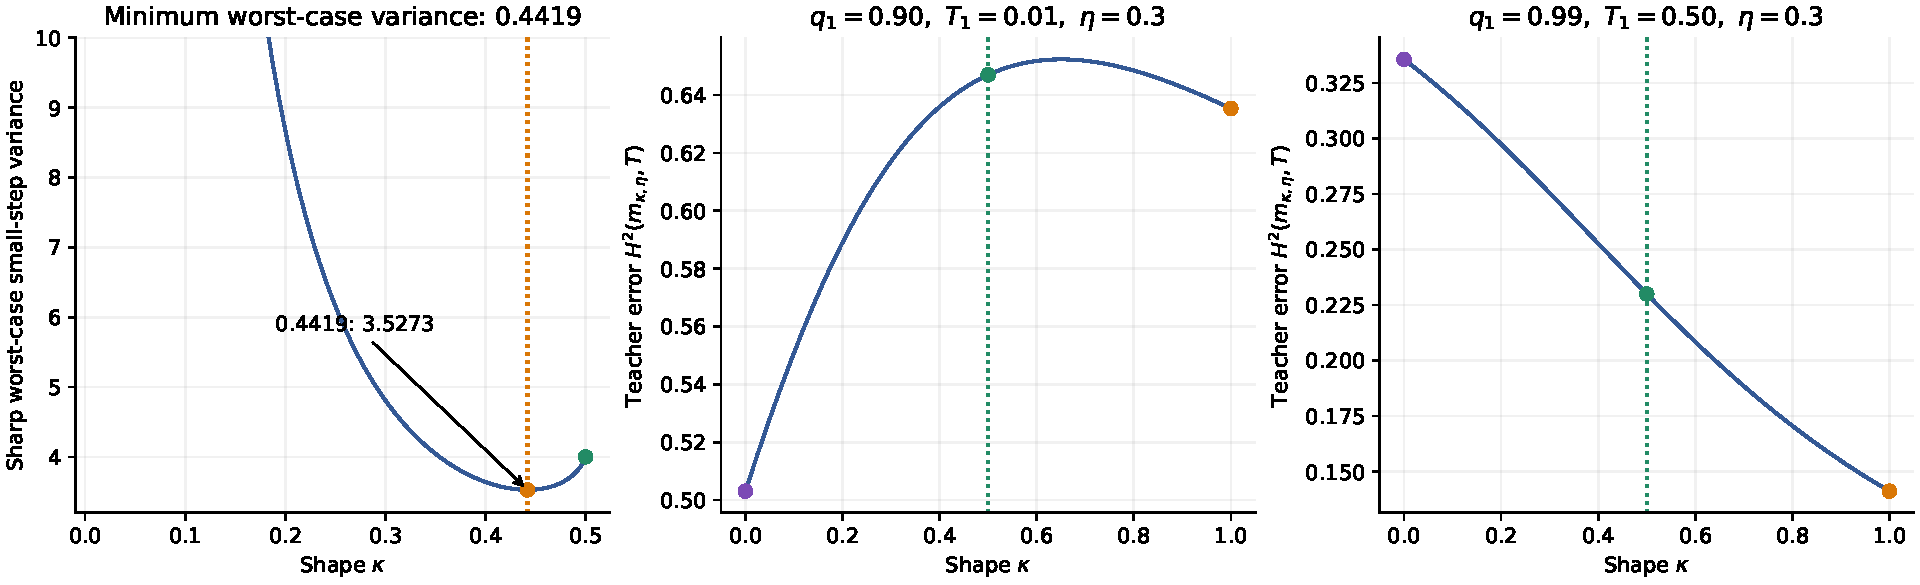
\includegraphics[width=\textwidth]{../../results/chapter9-restructure/kappa-criteria.pdf}
 \caption{形状的优势取决于评价标准。左图为锐最坏小步方差常数，最小点约为 $0.4419$，平方根点为 4。中、右图对同一 $\eta=0.3$ 使用两对固定二元分布，比较精确 target 后的同一 Hellinger 误差；曲线没有一致的形状排名。图只计算解析概率公式，不使用模型训练。}
 \label{fig:power-kappa-criteria}
\end{figure}

学生和教师的加权分布还可以用作辅助 action 提案，例如 $\mu_\zeta=(1-\zeta)q+\zeta T$。这与平方根监督 target 是两个选择：前者通过重要性校正估计原 $q$ 加权 BPO 损失，后者改变要拟合的目标。提案混合能控制重要性比率并在一些稀有 action 输入上改善相对方差，但没有每个输入都降低方差的保证。第~\ref{sec:power-estimators}~节给出无偏性、反例和排除重复 action 后的协方差半正定改进。
